% `template.tex', a bare-bones example employing the AIAA class.
%
% For a more advanced example that makes use of several third-party
% LaTeX packages, see `advanced_example.tex', but please read the
% Known Problems section of the users manual first.
%
% Typical processing for PostScript (PS) output:
%
%  latex template
%  latex template   (repeat as needed to resolve references)
%
%  xdvi template    (onscreen draft display)
%  dvips template   (postscript)
%  gv template.ps   (onscreen display)
%  lpr template.ps  (hardcopy)
%
% With the above, only Encapsulated PostScript (EPS) images can be used.
%
% Typical processing for Portable Document Format (PDF) output:
%
%  pdflatex template
%  pdflatex template      (repeat as needed to resolve references)
%
%  acroread template.pdf  (onscreen display)
%
% If you have EPS figures, you will need to use the epstopdf script
% to convert them to PDF because PDF is a limmited subset of EPS.
% pdflatex accepts a variety of other image formats such as JPG, TIF,
% PNG, and so forth -- check the documentation for your version.
%
% If you do *not* specify suffixes when using the graphicx package's
% \includegraphics command, latex and pdflatex will automatically select
% the appropriate figure format from those available.  This allows you
% to produce PS and PDF output from the same LaTeX source file.
%
% To generate a large format (e.g., 11"x17") PostScript copy for editing
% purposes, use
%
%  dvips -x 1467 -O -0.65in,0.85in -t tabloid template
%
% For further details and support, read the Users Manual, aiaa.pdf.


% Try to reduce the number of latex support calls from people who
% don't read the included documentation.
%
\typeout{}\typeout{If latex fails to find aiaa-tc, read the README file!}
%

\documentclass[]{aiaa-tc}% insert '[draft]' option to show overfull boxes

\usepackage{varioref}%  smart page, figure, table, and equation referencing
\usepackage{wrapfig}%   wrap figures/tables in text (i.e., Di Vinci style)
\usepackage{threeparttable}% tables with footnotes
\usepackage{dcolumn}%   decimal-aligned tabular math columns
\newcolumntype{d}{D{.}{.}{-1}}
\usepackage{nomencl}%   nomenclature generation via makeindex
\makeglossary
% \usepackage{subfigure}% subcaptions for subfigures
% \usepackage{subfigmat}% matrices of similar subfigures, aka small mulitples
\usepackage{subcaption}
\usepackage{fancyvrb}%  extended verbatim environments
\fvset{fontsize=\footnotesize,xleftmargin=2em}
\usepackage{lettrine}%  dropped capital letter at beginning of paragraph
\usepackage[colorlinks]{hyperref}%  hyperlinks [must be loaded after dropping]

% Ignore spaces in filenames
\usepackage[space]{grffile}
\usepackage{booktabs}

\title{Real-Time Performance Feedback in a \\Manually-Controlled Spacecraft Inspection Task}

\author{
John A. Karasinski%
  \thanks{Graduate Student Researcher, Mechanical and Aerospace Engineering, Student Member AIAA.}
\ and Stephen K. Robinson\thanks{Director – UC Davis Center for Human/Robotics/Vehicle Integration and Performance, Professor – Mechanical and Aerospace Engineering, Member AIAA.}\\
{\normalsize\itshape
 University of California, Davis, Davis, CA 95616}\\
\and
Patrick Handley%
  \thanks{Technical Staff, Member AIAA.}
\ and Kevin R. Duda\thanks{Principal Aerospace Human Factors Engineer, Member AIAA.}\\
{\normalsize\itshape
 Charles Stark Draper Laboratory, Cambridge, MA 02139}\\
}

% Data used by 'handcarry' option if invoked
\AIAApapernumber{YEAR-NUMBER}
\AIAAconference{Conference Name, Date, and Location}
\AIAAcopyright{\AIAAcopyrightD{YEAR}}

% Define commands to assure consistent treatment throughout document
\newcommand{\eqnref}[1]{(\ref{#1})}
\newcommand{\class}[1]{\texttt{#1}}
\newcommand{\package}[1]{\texttt{#1}}
\newcommand{\file}[1]{\texttt{#1}}
\newcommand{\BibTeX}{\textsc{Bib}\TeX}

\begin{document}

\maketitle

\begin{abstract}
  While operating a vehicle, well trained operators already know how to fly, but their performance can still be improved with the assistance of an expert providing feedback in real-time. Rather than focusing on the final results of a mission, real-time operator monitoring can produce an assessment of an operator's state and task performance. This, in turn, provides important context for interpreting the operator's actions and is critical for presenting timely and relevant feedback to the operator. We designed an automated flight instructor to provide real-time feedback to a human operator during a simulated Simplified Aid For EVA Rescue (SAFER) flight task. SAFER is a small propulsive jet pack worn during spacewalks for self-rescue~\cite{safer}. We investigate the effect of three variations of an instructor-model performance-feedback strategy on human performance in a novel SAFER inspection task. Real-time feedback was found to have a statistically significant effect of improving subject performance and decreasing workload in this complicated four degree of freedom manual control task with two secondary tasks.
\end{abstract}

\section{Motivation}
\lettrine[nindent=0pt]{W}{e}
%We
consider the distinction between guidance --- the information an operator receives about the vehicle's state, and performance feedback --- additional information that an instructor provides while training an operator. Guidance is the process of collecting and applying information for the purpose of generating maneuver commands to control vehicle movements~\cite{draper1965guidance}. In aerospace vehicles, guidance is usually presented to a pilot by visual displays which could include any number of changing numbers, words, lines, or other shapes. In contrast to guidance, feedback should act as an easily-accessible indicator of performance. Guidance already tells the pilot what to do --- feedback should simply inform them if they're following guidance well enough.

% \lettrine[nindent=0pt]{D}{espite}
Despite careful planning, extensive training, and the use of tethers, separation from spacecraft remains one of the greatest dangers during an extravehicular activity (EVA)~\cite{handley2014pilot}. Due to the time constraints imposed by orbital mechanics and the relative lack of maneuverability of larger spacecraft, self-rescue is the only option in the event of a separation. The Simplified Aid For EVA Rescue (SAFER) is a small propulsive jet pack worn by U.S. astronauts during spacewalks for contingency self-rescue~\cite{safer}. Prior to an EVA, SAFER is attached to the astronaut's Extravehicular Mobility Unit (EMU), and fulfills the need for a propulsive self-rescue system. SAFER remains inert during a nominal EVA, and is only deployed during a self-rescue event, see Figure~\ref{fig:safer_hardware}.

SAFER consists of several subsystems, including: propulsion, battery pack, avionics, sensors, and a hand controller. There are 24 fixed-position thrusters that exert forces on the astronaut for maneuvering in six degrees-of-freedom. The thrusters are controlled by on/off valves, which result in a bang-bang control scheme, and cannot be throttled~\cite{handley2014pilot}. The Hand Controller Module (HCM) includes a four degree-of-freedom joystick used to input astronaut commands and a switch to toggle between translation and rotation modes. Only one command can be executed at any time, placing further limits on control. The astronaut inputs commands into the HCM, and SAFER avionics software translates the commands into thruster outputs. Additional the details of these subsystems can be found in the SAFER Operations Manual~\cite{safer}.

NASA astronauts spend hundreds of hours training to use SAFER with expert instructors before flight. Training to proficient performance on this complex flight vehicle requires real-time feedback from an expert instructor. Training time and instructor availability are limited, however, and it is not easy to judge one's own performance during training flights due to the lack of any guidance or navigational feedback system. SAFER is flown entirely by hand and eyes. For the sake of this research, and looking forward to future improvements, we added a flight-guidance display for the SAFER pilot. From our pilot experiments, we designed a real-time performance feedback cue inspired by flight instructor function to provide feedback to a human subject during a simulated SAFER flight task~\cite{karasinski2016development}. We investigated the effects of three variations of instructor-model performance feedback on human performance in a novel SAFER inspection task.

\begin{figure}[tb!]
  \centering
  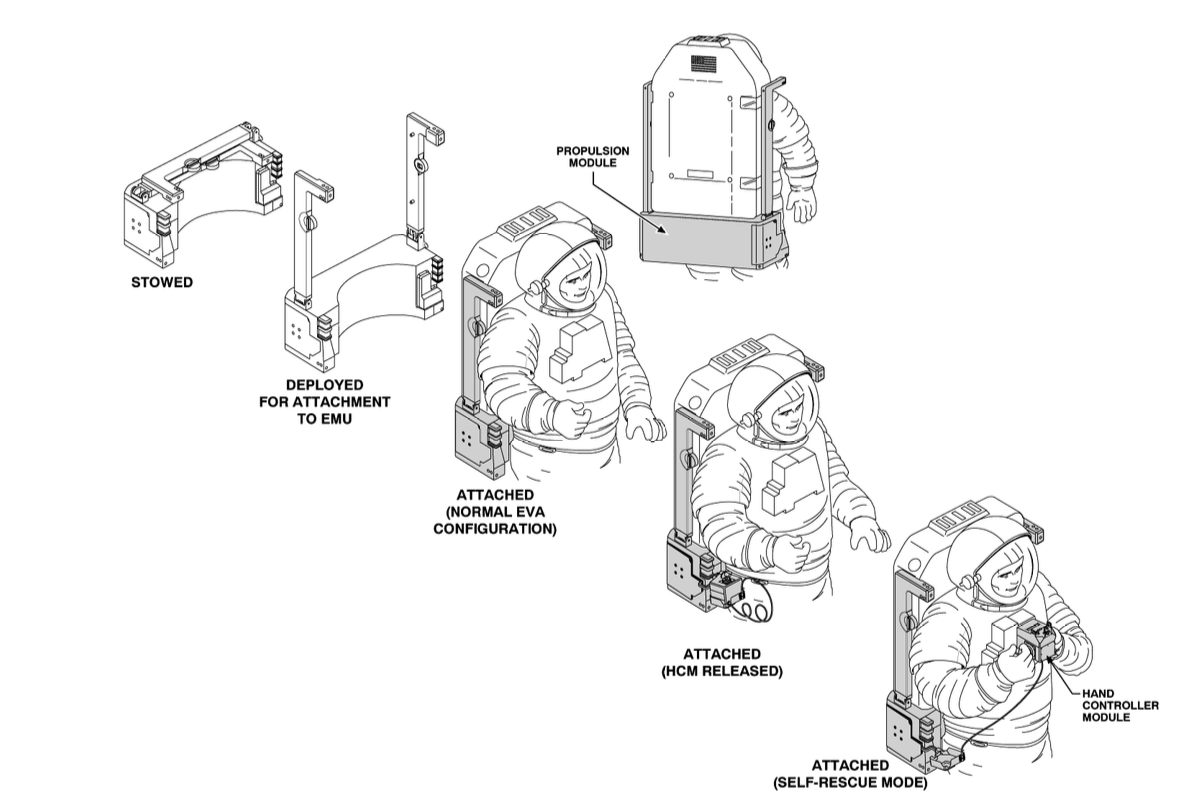
\includegraphics[width=0.8\linewidth]{figs/SAFER_diagram.png}
  \caption{Attachment of SAFER to EMU.~\cite{safer}}
  \label{fig:safer_hardware}
\end{figure}

\section{Experimental Design and Procedures}

\begin{figure}[tb!]
  \centering
  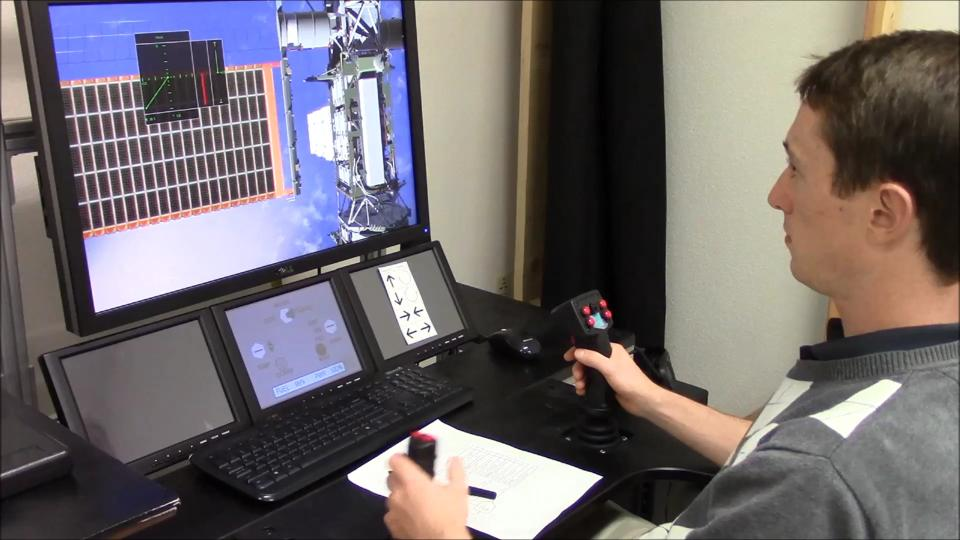
\includegraphics[width=0.8\textwidth]{figs/SAFER_DangerChris.jpg}
  \caption[An example subject sitting at the simulator grasping both controllers]{An example subject sitting at the simulator grasping both controllers. The out-the-window display with guidance in show on the large display, and the secondary display with mode and fuel indicators is on the middle display on the bottom. A controller cue card was available on the bottom right display to instruct the subjects how to use the controllers.}
  \label{fig:safer_subject}
\end{figure}

A human-in-the-loop simulation was conducted using a fixed-base simulator, see Figure~\ref{fig:safer_subject}. Subjects were instructed for approximately forty-five minutes prior to flights. Slides were presented from the experimenter's laptop, and pre-recorded audio was played on each slide, to ensure that each subject received identical training instructions. After the training, subjects flew with the experimenter on two practice flights to ensure their understanding of the task, task priorities, and use of the joysticks, as described below. A cue card explaining the controller commands was available in front of the subjects during both the training and during the experimental trials. Subjects were allowed to ask questions during the presentation of the slides and the practice flights, but not once the experiment had started.

Subjects manipulated two hand controllers to emulate the functions of SAFER's HCM. In this experiment, subjects are responsible for four degrees of freedom--three translational degrees and roll. The roll axis is defined relative to the plane of the solar array. The left joystick switched between translation and rotation modes, and had a thumb-activated side button to trigger a ``camera'' to take pictures of the damaged waypoints. Subjects used the right joystick to control three translational degrees of freedom while in translation mode, and roll (only) while in rotation mode (pitch and yaw could not be controlled by the subject, and were instead controlled by an autopilot which negated the effects of cross-coupling). The right joystick could be moved forwards/backwards, left/right, and twisted clockwise/counterclockwise.

Subjects used the two vertically arranged displays in the simulator to complete the task, see Figure~\ref{fig:safer_subject}. The primary display contained an out-the-window view of the solar array and, depending on which group the subject was in, one of the guidance displays from Figure~\ref{fig:displays}. Subjects used the out-the-window view and guidance display to navigate their environment. The secondary display located directly below the primary display displayed information about the subject's current mode, remaining fuel, and a `comm light'. Subjects developed a scan pattern during training on the task, as they were required to use information from both displays to complete the experiment. No scan strategy was suggested during the training, and subjects were allowed to develop any strategy that they deemed most effective.

Subjects were tasked with flying SAFER to perform an inspection of the International Space Station's (ISS) solar arrays. An example side view of the task can be seen in Figure~\ref{fig:safer_demo}. Subjects were initially placed 40 feet away from the solar array, and were asked to close to 30 feet and hold this distance for the remainder of the task. Subjects could gauge their distance from the solar array using the indicator on the guidance display. Subjects were then asked to inspect 4 ``damaged'' points on the solar array, and were given a guidance display for navigation to the waypoints, see Figure~\ref{fig:displays}. We also implemented an unexpected waypoint redesignation during half the trials. When this occurred, one of the waypoints would be updated to a new location while the subject was in mid-flight toward the original waypoint. Subjects were notified of this change with an audible ``ding'', and the guidance display updated instantaneously. If the trial had an waypoint redesignation on the second waypoint, for instance, the subject would: close from 40 feet to 30 feet, use the guidance to fly towards the first waypoint and inspect, use the guidance to fly towards the second waypoint, hear the audible ``ding'' and guidance display changes and readjust their trajectory, inspect the waypoint, fly to third waypoint and inspect, and fly to the fourth waypoint and inspect.

The manual-control task consisted of, in order of priority:
\begin{enumerate}
  \itemsep0em
  \item Maintaining the distance from the solar array at 30 feet
  \item Minimizing the roll angle to a relative angle of 0 degrees to the solar array
  \item Navigating the waypoints as quickly and accurately possible
\end{enumerate}

\begin{figure}[tb!]
  \centering
  \begin{subfigure}{.5\textwidth}
    \centering
    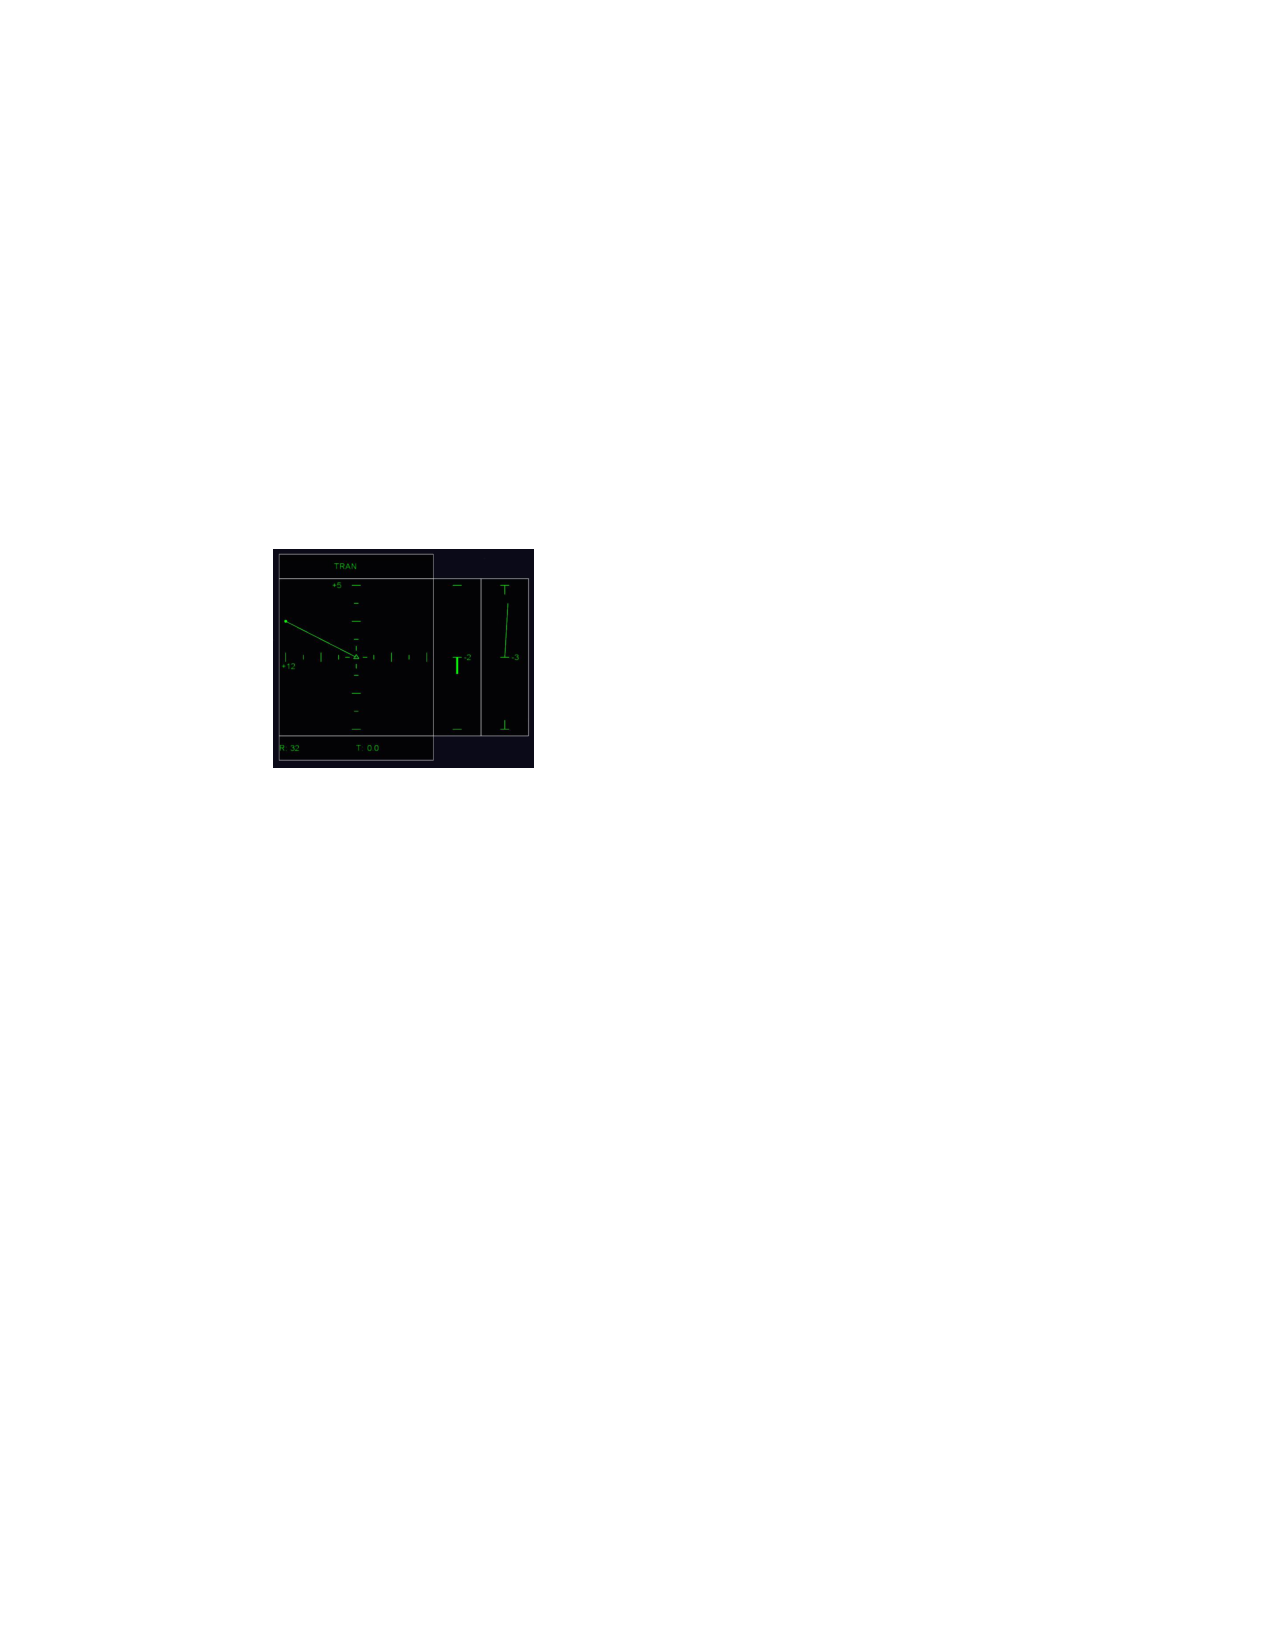
\includegraphics[width=.99\linewidth, page=1]{figs/guidance_full.pdf}
    \caption{Group 1 -- Control}
    \label{fig:sub1}
  \end{subfigure}%
  \begin{subfigure}{.5\textwidth}
    \centering
    \includegraphics[width=.99\linewidth, page=2]{figs/guidance_full.pdf}
    \caption{Group 2 -- Decimal}
    \label{fig:sub2}
  \end{subfigure}\vspace{1em}
  \begin{subfigure}{.5\textwidth}
    \centering
    \includegraphics[width=.99\linewidth, page=3]{figs/guidance_full.pdf}
    \caption{Group 3 -- Color}
    \label{fig:sub2}
  \end{subfigure}
  \caption{Guidance displays for all three groups in the same simulation state.}
  \label{fig:displays}
\end{figure}

\begin{figure}[tb!]
  \centering
  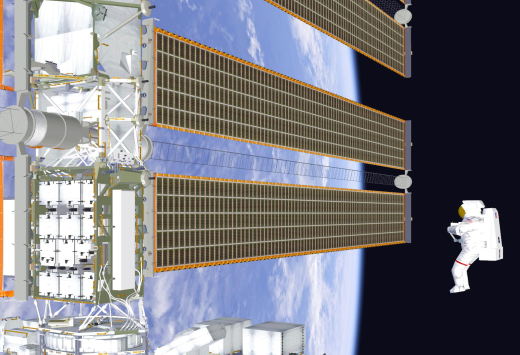
\includegraphics[width=0.8\linewidth]{figs/safer_visual.png}
  \caption{Example side view of the SAFER inspection task flown by the subjects in this experiment.}
  \label{fig:safer_demo}
\end{figure}

While performing the flying task, subjects were also asked to respond to a secondary task in the form of a ``comm light''~\cite{crosby1979dual, wickens1986sternberg, hainley2013pilot}. This light, a colored concentric circle on the secondary display, changed from a teal color to a blue or a green color every 5 to 7 seconds (at a pseudorandom interval), and the subjects responded by pressing the corresponding button on the joystick. This secondary task was displayed on a separate screen from the flight tasks, and the change in color could not be easily distinguished from the subjects' peripheral vision, requiring the subjects to establish a visual scan pattern that included information on both primary and secondary displays. Response time to this two-choice secondary task was used as an objective measure subject's workload. After each trial, subjects were also asked to rate their workload using the Modified Bedford Workload Scale, as a subjective measurement of their workload~\cite{wickens1991processing}. Finally, the subjects made verbal callouts about their fuel level every 5\% (e.g., 95\%, 90\%, 85\%, ...), which provided an indication of their situational awareness. Subjects were pseudo-randomly assigned into one of three groups, and each subject flew a total of 22 trials. The first two training trials were flown with instruction from the experimenter to insure that the subjects had no remaining questions about how to fly or how the controls worked. Subjects were allowed to ask questions during this time, and these trials were not used in any analysis. Experimental trials 1-10 and trials 11-20 used the same set of waypoints, see Table~\ref{tab:all_trials}.

\begin{table}[tb!]
  \centering
  \begin{tabular}{rrrrr}
    \toprule
    Group & Name    & Analog Display Max & Significant Figures & Color Feedback \\
    \midrule
    1     & Control & 10 (ft)            & 1                   & No             \\
    2     & Decimal & 5 (ft)             & 2                   & No             \\
    3     & Color   & 10 (ft)            & 1                   & Yes            \\
    \bottomrule
  \end{tabular}
  \caption{Experimental differences between subject groups}
  \label{tab:group_diffs}
\end{table}

\begin{table}[b]
  \begin{center}
    \begin{tabular}{cc|cc|cc|cc}
      \toprule
      Trial & Ad-hoc & Trial & Ad-hoc & Trial & Ad-hoc & Trial & Ad-hoc \\
      \midrule
      1     & N      & 6     & Y$^4$  & 11    & N      & 16    & Y$^4$  \\
      2     & Y$^2$  & 7     & Y$^2$  & 12    & Y$^2$  & 17    & Y$^2$  \\
      3     & N      & 8     & N      & 13    & N      & 18    & N      \\
      4     & Y$^3$  & 9     & N      & 14    & Y$^3$  & 19    & N      \\
      5     & N      & 10    & Y$^3$  & 15    & N      & 20    & Y$^3$  \\
      \bottomrule
    \end{tabular}
  \end{center}
  \caption{The order of trials is the same among all subjects. Trials either had no ad-hoc redesignation (N), or had a redesignation on waypoint number $X$ (Y$^X$).}
  \label{tab:all_trials}
\end{table}

As a result of the guidance display treatments (control, decimal, color), subjects within a group experienced different real-time feedback, see Figure~\ref{fig:displays} and Table~\ref{tab:group_diffs}. Group 1 acted as a control group, and had an analog distance display that read from -10 to 10 feet, and digital displays with one significant figure (e.g., 1, 2, 3...). Group 2 had an analog distance display that read from -5 to 5 feet, and digital display with two significant figures (e.g., 1.2, 2.7, 9.4) for distance and roll. Group 3 had the same analog and digital distance displays as Group 1, and experienced real-time feedback in the form of distance and roll displays that changed color. When the instantaneous error rose above a threshold value which we chose, the appropriate display changed from green to red. These displays are decoupled, and were activated independently of each other. Group 3 had distance feedback parameter of 1 foot, and a roll feedback parameter of 1.35 degrees, the asymptotic limit of Group 1.

\section{Research Questions and Hypotheses}
Under the guiding principle that an experienced flight instructor can lead to a better trained student, we sought to answer the following questions:

\begin{enumerate}
  \itemsep0em
  \item Can subjects' fully trained performance level be increased with the use of real-time performance feedback based on our "instructor model"? Subjects presented with the feedback are referred to as being in a treatment group. We expect that subjects in the two treatment groups will have a lower mean absolute distance error, mean absolute roll error, and a lower task completion time. This expectation arises from the preliminary results, and anecdotal evidence of improved performance of students in the presence of flight instructors~\cite{karasinski2016development}.
  \item Can subjects' workload be decreased with the use of real-time performance feedback? We expect that subjects in the color based real-time feedback group will report lower workload and respond to the secondary task more often. The real-time performance feedback should shift some workload from the subject onto the computer, allowing the subject more time to respond to the secondary task.
  \item Can subjects' training time be decreased with the use of real-time performance feedback? We expect the learning rates of subjects in the two treatment groups to increase. Anecdotal evidence suggests that experienced flight instructors can produce well trained students in shorter periods of time.
\end{enumerate}

\section{Subject Demographics}
A human-in-the-loop simulation was conducted to gather data from 30 subjects (26 males, 4 females), with an average age of $21.9\pm3.7$ years ($21.8\pm3.7$ years for males, $22.0\pm4.6$ years for females). Subjects were undergraduate and graduate students in the UCD School of Engineering. Out of the 30 subjects, 23 were undergraduate students, and 7 were graduate students. Additionally, 19 subjects had previous experience with a flight simulator, 3 subjects were pilots, and 1 subject was training for their pilot's license. Though not a requirement for the experiment, all subjects were right handed. Females and pilots were assigned to groups such that their presence in each group was as balanced as possible--there were 2 females in Groups 1 and 2, and 3 females in Group 3 and there was 1 pilot in each group.

\section{Experimental Results}
Subject performance was quantified by recording the mean absolute error between the the required distance and roll, and by measuring the trial completion time. Secondary task response rate and modified Bedford scores were also analyzed. The main differences between the groups can be seen in Table~\ref{tab:group_diffs}.

Experimental results suggest that Groups 2 and 3 both performed better than the control group on the primary and secondary flight tasks, see Figure~\ref{fig:performance}. From the very first trial, subjects in Group 3 were able to perform better than Group 1 could at the end of the experiment. This suggests that the real-time performance feedback immediately provided a performance improving effect, even with novice subjects. Subjects in the feedback group (Group 3) also reported the lowest levels of workload via their post-trial Modified Bedford Workload scores, see Figure~\ref{fig:workload}. While both Groups 2 and 3 showed performance improvements over the control group, Group 2's workload was increased, as was their time to complete the task. Group 3 showed even larger performance improvements than Group 2, and also showed lower workload levels and only marginally larger time to complete the task.

One-way ANOVAs were run the on the data collected from Trials 11-20, when subjects were at or near their final performance level and learning effects were minimal~\cite{fisher1925statistical}. The results from each subject's second set of 10 trials were averaged, and five ANOVA's were run to test the effect of experimental group for significance at a level $\alpha = 0.05/5 = 0.01$ level. One-way ANOVA tests the null hypothesis that two or more groups have the same population mean. Tukey honest significant different post-hoc pairwise comparisons were Bonferroni-corrected~\cite{tukey1949comparing}. With the exception of workload, four of the five ANOVAs reported significant findings at the $\alpha = 0.01$ level. The results of the ANOVAs and post-hoc tests are listed in the sections below. These ANOVAs are reported with three values, $F$, $df$, and $p$. $F$ is the F-statistic --- the ratio of the variance calculated among the means to the variance within the samples, $df$ is the degrees of freedom, and $p$ is the probability that the result of the F-test and degrees of freedom is the same as or more extreme than the actual observed results~\cite{wasserstein2016asa}.

\subsection{Flight Performance}
Significant effects were seen between Groups 1 and 3 for both the mean absolute distance error ($F=6.292$, $df = 2$, $p = 0.005$) and mean absolute roll error ($F=8.348$, $df = 2$, $p = 0.001$), suggesting that the use of real-time feedback improved performance. In regards to our first hypothesis, \textit{Can subjects' fully trained performance level be increased with the use of real-time performance feedback?}, we find: Yes, real-time performance feedback can improve subjects' fully trained performance levels. It remains unclear, however, why the real-time feedback improves performance, though it is likely that the change in display color acts as an effective gaze attractor (see Wickens and Hollands~\cite{wickens2015engineering}). The change in color may cause subjects to shift their gaze back to the indicator, and may also act as a scan-repair tool for subjects who had stopped checking the indicator. %See Tables~\ref{tab:performance_anova} and~\ref{tab:performance_tukey} for the complete statistical results for distance, and Tables~\ref{tab:roll_anova} and~\ref{tab:roll_tukey} for the results for roll.

A significant increase in time ($F=7.557$, $df = 2$, $p = 0.002$) was seen in Group 2 over Group 1, suggesting that giving subjects an extra decimal place of information caused the subjects to fly more slowly. These subjects may have been spending so much time on their primary and secondary tasks that they did not have enough to to attend to their tertiary task of flying to the waypoints. This was experienced with a small number of people during software debugging sessions during the development of the simulation. %See Tables~\ref{tab:time_anova} and~\ref{tab:time_tukey} for the complete statistical results.
This was an expected effect from early testing of the simulator, where users were observed to spend more time viewing the indicator than monitoring the other instruments.

Exponential fits can be used to model the subject's learning rate throughout the 20 trials.\begin{equation}
E_i = A e^{(-i/B)} + C
\label{onlyequation}
\end{equation}
where $E_i$ was the trajectory error for the trial i within a training or washout phase, $A$ is the amount of learning (the change of the trajectory errors due to training), $B$ is the time constant indicating the number of trials for the error to decrease 67\% of the way to asymptote, and $C$ is the asymptotic (steady-state) error value.

To investigate whether subject's learning time could be decreased, Equation~\ref{onlyequation} was used. To investigate the effect of group on learning times, we calculate the best exponential fit for the primary flight task. The results for these fits can be seen in Table~\ref{tab:dist_exp_fits}. While the difference in learning rates (B) among the three groups is minimal, both the amount of learning (A) and the steady state error (C) values are very different. The amount of learning in Groups 2 and 3 is less than half of Group 1, and the steady state error value for Group 3 is more than 40\% lower than that of Group 1. In regards to our third hypothesis, \textit{Can subjects' training time be decreased with the use of real-time performance feedback?}, we find: Subjects receiving our instructor-model real-time performance feedback require a similar number of trials to reach their final performance level, but require less time to meet minimum performance requirements. While the learning rate is not very different among the three groups, the average improvement from trial to trial is much lower for subjects in Group 3 compared to Group 1. As both the initial and steady state performance is significantly better for Group 3 than Group 1, the amount of trial-to-trial improvement for subjects in Group 3 was much smaller than Group 1.

\begin{table}[tb!]
  \centering
  \begin{tabular}{rrrr}
    \toprule
    Group & $A$ (Feet) & $B$ (Trials) & $C$ (Feet) \\
    \midrule
    1     & 1.16       & 4.80         & 0.69       \\
    2     & 0.55       & 3.60         & 0.60       \\
    3     & 0.43       & 4.49         & 0.38       \\
    \bottomrule
  \end{tabular}
  \caption[Results of fitting the mean absolute distance error to an exponential model for each group]{Results of fitting the mean absolute distance error to an exponential model for each group. Values are the fit values for Equation~\ref{onlyequation} ($E_i = A e^{(-i/B)} + C$). $E_i$ was the trajectory error for the trial i within a training or washout phase, $A$ is the amount of learning (the change of the trajectory errors due to training), $B$ is the time constant indicating the number of trials for the error to decrease 67\% of the way to asymptote, and $C$ is the asymptotic (steady-state) error value.}
  \label{tab:dist_exp_fits}
\end{table}

\begin{figure}[tb!]
  \centering
  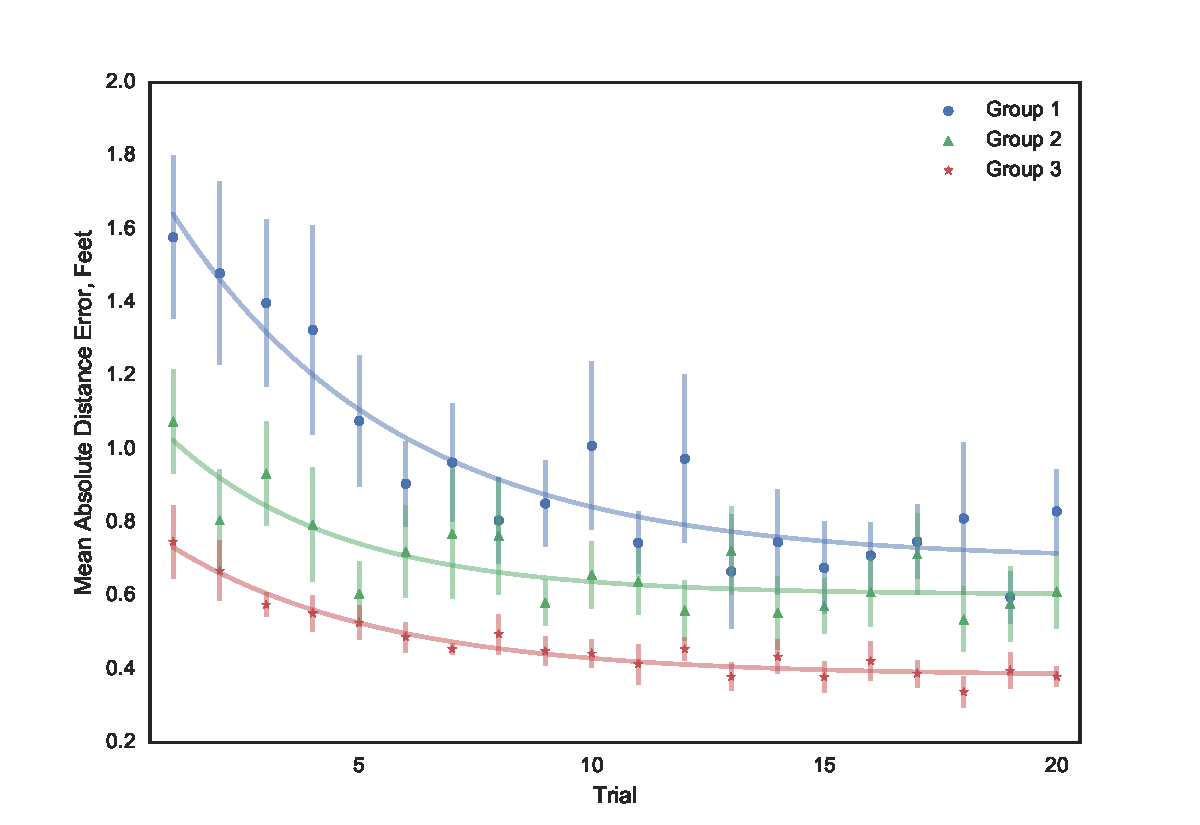
\includegraphics[width=0.8\linewidth]{figs/Group_absDistErr_clean_fit_30.pdf}
  \caption[Mean absolute distance error from the solar array per trial]{Mean absolute distance error from the solar array in feet per trial. Data points show the mean; error bars are the standard error of the mean. Lines show exponential fits to the values by trial, see Equation~\ref{onlyequation}. All subject group show a large amount of learning during the first half of the experiment, then settle to a steady state value.} \label{fig:performance}
\end{figure}

\begin{figure}[tb!]
  \centering
  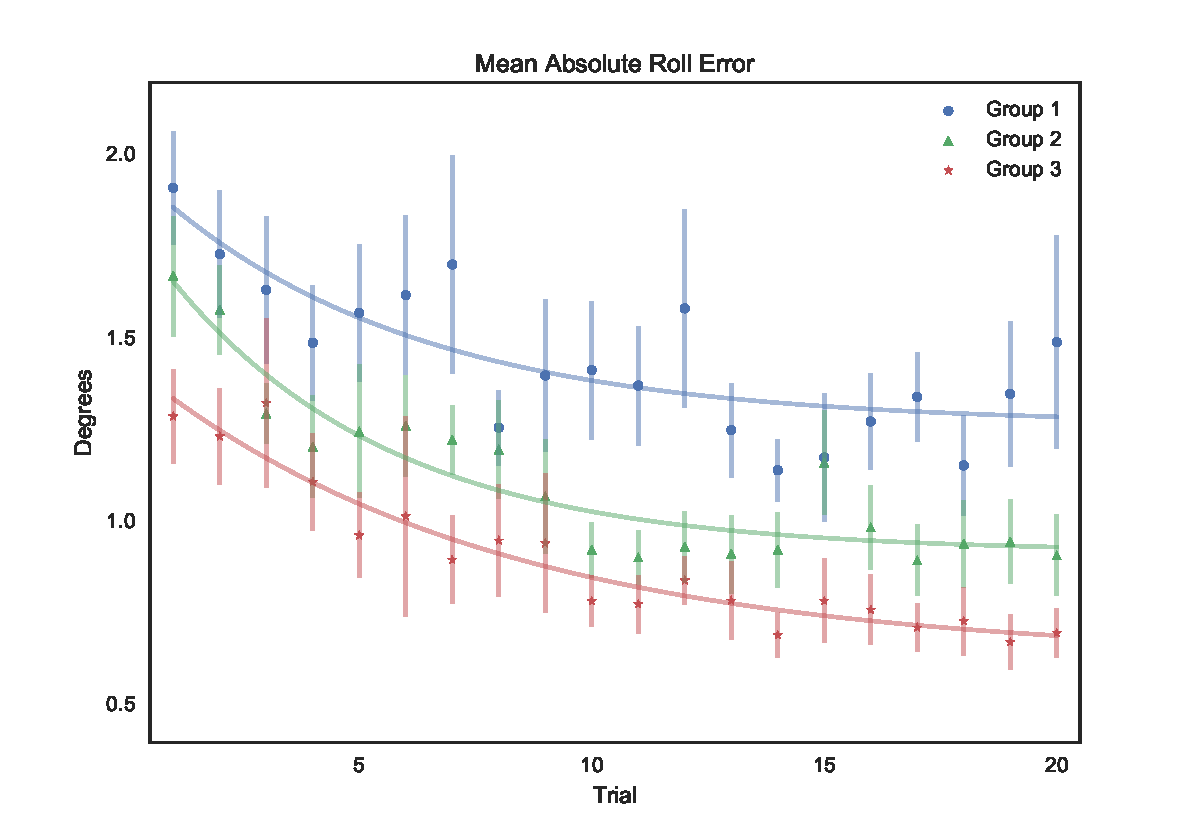
\includegraphics[width=0.8\linewidth]{figs/Group_absRollErr_clean_fit_30.pdf}
  \caption[Mean absolute roll error in degrees per trial]{Mean absolute roll error in degrees per trial. Data points show the mean; error bars are the standard error of the mean. Lines show exponential fits to the values by trial, see Equation~\ref{onlyequation}.}
  \label{fig:roll}
\end{figure}

% \begin{figure}[tb!]
%   \centering
%   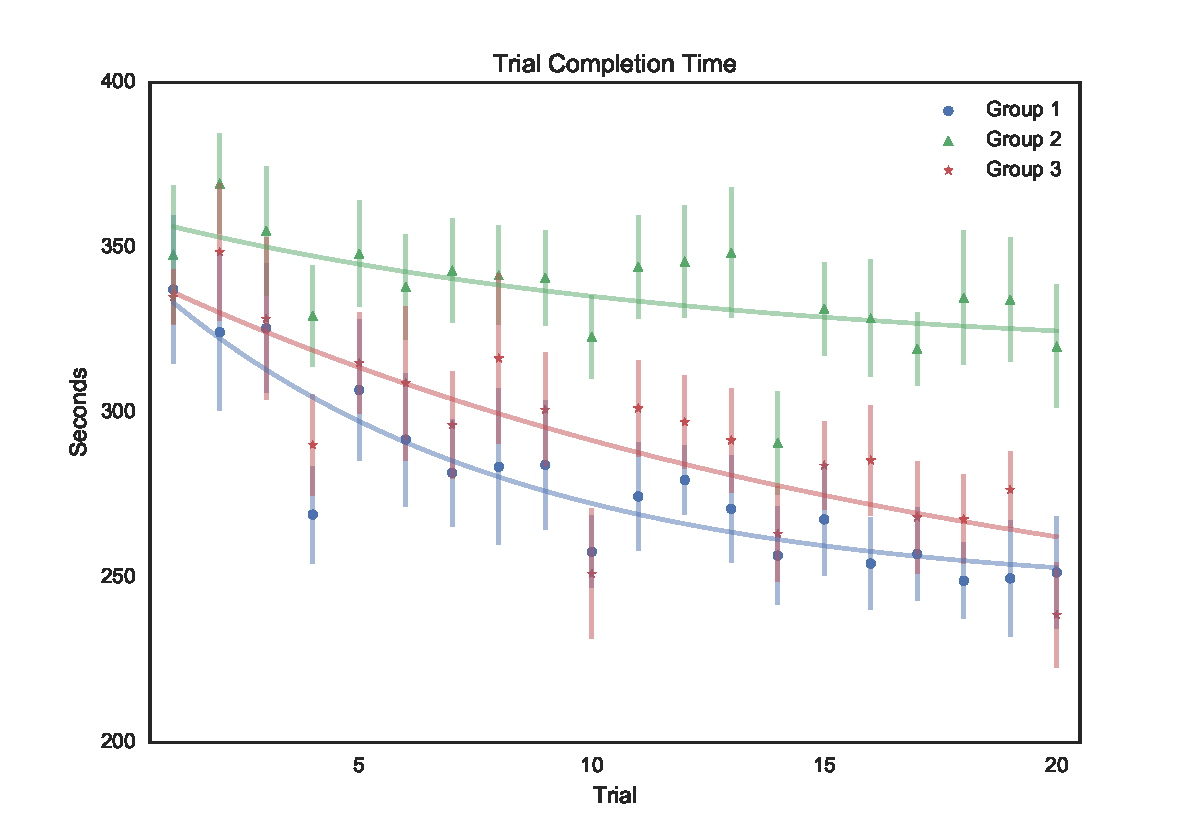
\includegraphics[width=0.8\linewidth]{figs/Group_Time_fit_30.pdf}
%   \caption[Mean time to complete the task, in seconds, per trial]{Mean time to complete the task, in seconds, per trial. Data points show the mean; error bars are the standard error of the mean. Lines show exponential fits to the values by trial, see Equation~\ref{onlyequation}.}
%   \label{fig:time}
% \end{figure}

\subsection{Secondary Task Response Rate}
There were significant differences between Groups 1 and 2, and between Groups 2 and 3 for the percentage of secondary tasks completed ($F=14.859$, $df = 2$, $p < 0.001$).%, see Tables~\ref{tab:secondary_anova} and~\ref{tab:secondary_tukey}.
Group 2 completed significantly fewer secondary tasks than Group 1, while Group 3 completed significantly more secondary tasks than Group 1. This is consistent with the results seen with respect to the time to complete the task, as subjects in Group 2 spent more time with the primary flight displays and less time with the secondary tasks than Group 1. As seen in Figure~\ref{fig:secondary}, subjects in groups 1 and 2 initially respond at the same rate, but separate out into individual lines as the experiment continues. Group 3, however, immediately responds to additional secondary tasks. Subjects may have relied upon the real-time feedback to spend more attention attending to the secondary task, as the feedback would attract their gaze back to the guidance display when they drifted too far off the primary tasks. This effect may have allowed subjects in Group 3 to be more attentive with the secondary task than those in Group 1.

\subsection{Subjective Workload}

\begin{figure}[tb!]
  \centering
  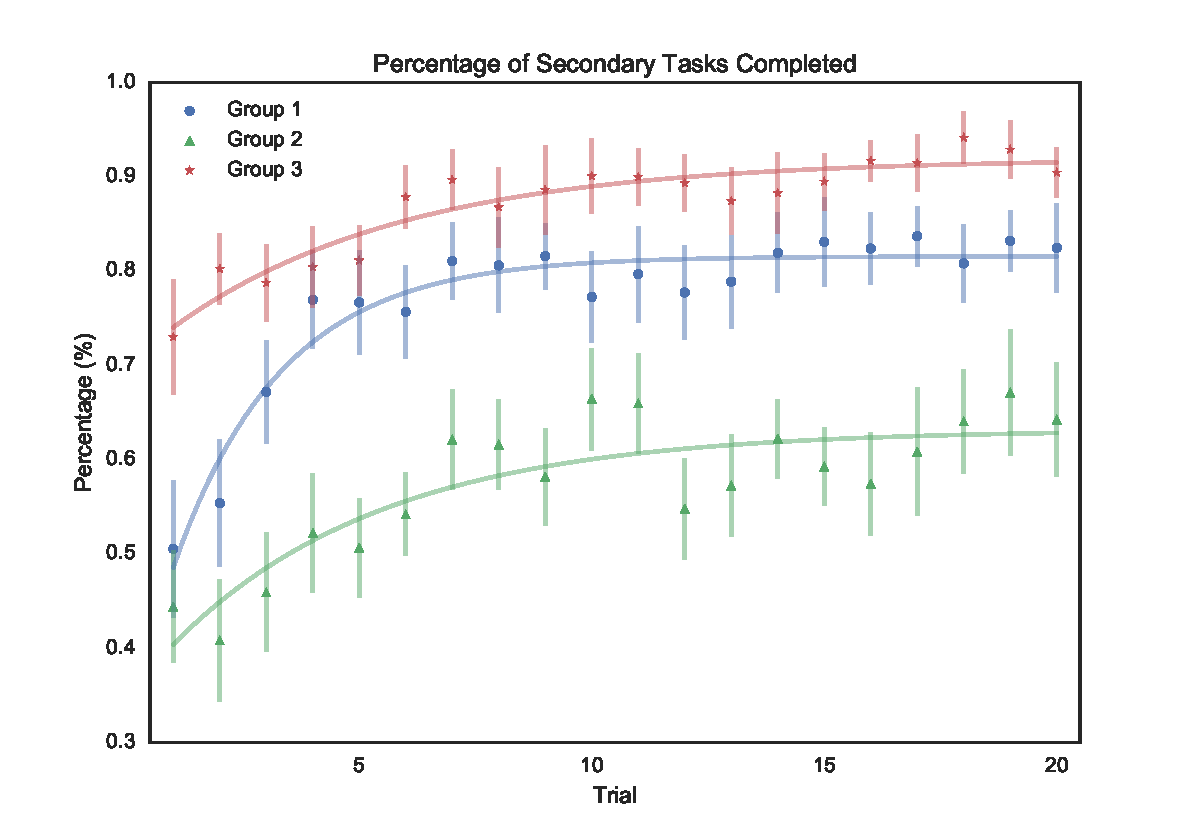
\includegraphics[width=0.8\linewidth]{figs/Group_Percentage_fit_30.pdf}
  \caption[Mean percentage of secondary tasks attended to within the 5 second timeout period per trial]{Mean percentage of secondary tasks attended to within the 5 second timeout period per trial. Data points show the mean; error bars are the standard error of the mean. Lines show exponential fits to the values by trial.}
  \label{fig:secondary}
  \vspace{1em}
\end{figure}

\begin{figure}[tb!]
  \centering
  \includegraphics[width=0.8\linewidth]{figs/Group_workload_fit_30.pdf}
  \caption[Mean self reported Modified Bedford Workload Score per trial]{Mean self reported Modified Bedford Workload Score per trial. Data points show the mean; error bars are the standard error of the mean. Lines show exponential fits to the values by trial. All subjects group initially report the same level of workload, but separate out into individual lines as the experiment continues.
  }
  \label{fig:workload}
\end{figure}

No significant effects were seen with respect to the self-reported Modified Bedford Scores ($F=4.157$, $df = 2$, $p = 0.026$).%, see Tables~\ref{tab:workload_anova} and~\ref{tab:workload_tukey}.
While subjects in all groups rated their initial workload similarly, they rated their fully-trained workload levels differently, see Figure~\ref{fig:workload}. Subjects in Group 2 reported the highest workload levels, followed by Group 1 and then Group 3. Despite this, we did not find statistically significant effects in either the ANOVA or Tukey HSD tests. In regards to our second hypothesis, \textit{Can subjects' workload be decreased with the use of real-time performance feedback?}, we find: Subjects receiving real-time performance report lower, though not statistically significant, levels of workload. Given the low $p$ value found by the ANOVA, however, it is possible that increasing the sample size by a few additional subjects could make this finding statistically significant.

\section{Discussion}

We investigated the effects of variations of an instructor-model performance feedback strategy on human performance in a novel SAFER inspection task. We hypothesized that real-time feedback would improve subject flight performance, decrease workload, and decrease training time. Results from this experiment indicate that at least one simple form of real-time feedback can improve subject flight performance and decrease workload. Whether training times can be reduced is still not clear. The rate at which subjects in all three groups learned was consistent, though the amount of learning happening on a trial-to-trial basis was different. Subjects in the real-time feedback group experienced lower trial-to-trial learning due to the groups initially superior performance.

In general, subjects in treatment Groups 2 and 3 had better performance in both the distance and roll tasks than subjects in the control group. Subjects in Group 3 had an \textit{initial} performance which was superior to the \textit{final} performance observed by subjects in Group 1. The magnitude of this effect surprising, and it appears to confirm that continuous, real-time feedback can greatly accelerate the learning of the task. ANOVA and post-hoc Tukey HSD tests showed that subjects in Group 3 had a better fully-trained performance level than subjects in Group 1, confirming our hypothesis. While the number of trials required to reach peak performance did not significantly vary among the three groups, subjects in Group 3 improved less on a trial-to-trial basis as their initial performance was superior. While subjective workload was not significantly different among any of the three groups, the subjects with feedback reported the lowest workload.

Decreasing workload, improving flight performance, and reducing training time can reduce operational costs and time, and improve crew safety.  While presenting more detailed numerical information on flight parameters can improve subject performance, we show that it does so at the cost of higher workload and longer task completion times compared to a control group. The use of real-time performance feedback to modify the guidance display was significantly effective at improving subject performance, and subjects also reported lower levels of subjective workload.

While different techniques for calculating when to provide and how to display feedback should be investigated, the technique used here proved simple and effective. The challenge with this technique is that it requires a predefined deadband for each flight mode. While this is easy to precalculate for simulators, real life scenarios do not always go as planned. Novel scenarios would require new feedback deadbands which may be nontrivial or impossible to calculate ahead of time. The choice of what value to choose for the deadband may not always be clear. While the value effectively sets a performance requirement on subjects, it likely has other effects on the subject's interpretation of task priority. If the performance requirements are driven too high they may sacrifice other tasks, and if the deadband is set too loose then the feedback is no longer useful as it will not occur. If the deadband is set too tight and the required performance cannot be achieved by dropping other tasks the subject could become frustrated with the feedback and ignore it entirely. This illustrates that a proper choice of deadband should be carefully considered, as setting too low or high performance requirements may lead to unpredicted or unexpected subject behavior.

One impressive thing to note, however, is that many subjects in the real-time feedback group did not use the feedback after they were several trials into the experiment. After the initial closing from 40 to 30 feet, several subjects never drifted back outside the 1 foot deadband around the 30-foot mark. As such, these subjects would have performed just as well if the feedback had been removed at that point. So, while it may not be practical to use this type of feedback mechanism outside of the training environment, it may be sufficient to supply subjects with feedback \textit{only} during training. Future research should investigate the effects of removing feedback from subjects.

While some prior research suggests that subjects can become dependent on the feedback mechanism instead of learning the task, this does not appear to be an issue here. Subjects tend to become dependent on the feedback when there is no other simple way to gauge task performance. In our experiment the guidance display is overlaid on the out-the-window view, and subjects may have been able to use this extra information to their advantage. While we cannot know where the subjects were looking during these flights, it may be that they were using out-the-window view to fly, and referencing back to the guidance display only when they noticed the change in color. This would suggest that the out-the-window display was sufficient to adequately fly the task, which makes sense when considering Figure~\ref{fig:safer_subject}. The out-the-window view primarily consists of the solar array, which is represented as a grid of uniform, well defined boxes. The size and relative angle of these boxes can be used in a way similar to the guidance display. Subjects that were not in the feedback group may not have been able to use this technique to fly as their performance never improved to similar levels as the real-time feedback group. This difference in strategy is promising, and should be investigated further.

% \begin{table}[h!]
%   \centering
%   \begin{tabular}{rrrrrr}
%     \toprule
%               & $df$ & $SS$  & $MS$  & $F$   & $p$   \\
%     \midrule
%     Group     & 2    & 0.058 & 0.029 & 6.292 & 0.005 \\
%     Residuals & 27   & 0.125 & 0.004 &       &       \\
%     \bottomrule
%   \end{tabular}
%   \caption{Mean absolute distance error one-way ANOVA of Groups results.}
%   \label{tab:performance_anova}
% \end{table}

% \begin{table}[h!]
%   \centering
%   \begin{tabular}{rrrrr}
%     \toprule
%     Group & Diff. Means & Lower  & Upper  & $p_{adj}$ \\
%     \midrule
%     2-1   & -0.042      & -0.117 & 0.033  & 0.365     \\
%     3-1   & -0.107      & -0.182 & -0.031 & 0.004     \\
%     3-2   & -0.065      & -0.140 & 0.010  & 0.100     \\
%     \bottomrule
%   \end{tabular}
%   \caption{Tukey HSD pairwise post-hoc comparisons for the mean absolute distance error one-way ANOVA of Groups results.}
%   \label{tab:performance_tukey}
% \end{table}

% \begin{table}[h!]
%   \centering
%   \begin{tabular}{rrrrrr}
%     \toprule
%               & $df$ & $SS$  & $MS$  & $F$   & $p$   \\
%     \midrule
%     Group     & 2    & 1.655 & 0.827 & 8.349 & 0.001 \\
%     Residuals & 27   & 2.676 & 0.099 &       &       \\
%     \bottomrule
%   \end{tabular}
%   \caption{Mean absolute roll error one-way ANOVA of Groups results.}
%   \label{tab:roll_anova}
% \end{table}

% \begin{table}[h!]
%   \centering
%   \begin{tabular}{rrrrr}
%     \toprule
%     Group & Diff. Means & Lower  & Upper  & $p_{adj}$ \\
%     \midrule
%     2-1   & -0.362      & -0.712 & -0.013 & 0.040     \\
%     3-1   & -0.568      & -0.917 & -0.218 & 0.001     \\
%     3-2   & -0.205      & -0.554 & 0.143  & 0.326     \\
%     \bottomrule
%   \end{tabular}
%   \caption{Tukey HSD pairwise post-hoc comparisons for the mean absolute roll error one-way ANOVA of Groups results.}
%   \label{tab:roll_tukey}
% \end{table}

% \begin{table}[h!]
%   \centering
%   \begin{tabular}{rrrrrr}
%     \toprule
%               & $df$ & $SS$  & $MS$  & $F$   & $p$   \\
%     \midrule
%     Group     & 2    & 26174 & 13087 & 7.557 & 0.002 \\
%     Residuals & 27   & 46758 & 1732  &       &       \\
%     \bottomrule
%   \end{tabular}
%   \caption{Time to complete the task one-way ANOVA of Groups results.}
%   \label{tab:time_anova}
% \end{table}

% \begin{table}[h!]
%   \centering
%   \begin{tabular}{rrrrr}
%     \toprule
%     Group & Diff. Means & Lower   & Upper   & $p_{adj}$ \\
%     \midrule
%     2-1   & 69.196      & 23.052  & 115.340 & 0.002     \\
%     3-1   & 16.293      & -29.850 & 62.437  & 0.660     \\
%     3-2   & -52.902     & -99.046 & -6.758  & 0.022     \\
%     \bottomrule
%   \end{tabular}
%   \caption{Tukey HSD pairwise post-hoc comparisons for the time to complete the task one-way ANOVA of Groups results.}
%   \label{tab:time_tukey}
% \end{table}

% \begin{table}[h!]
%   \centering
%   \begin{tabular}{rrrrrr}
%     \toprule
%               & $df$ & $SS$  & $MS$  & $F$    & $p$      \\
%     \midrule
%     Group     & 2    & 0.458 & 0.228 & 14.860 & $<$0.001 \\
%     Residuals & 27   & 0.416 & 0.015 &        &          \\
%     \bottomrule
%   \end{tabular}
%   \caption{Percentage of secondary tasks responded to per trial one-way ANOVA of Groups results.}
%   \label{tab:secondary_anova}
% \end{table}

% \begin{table}[h!]
%   \centering
%   \begin{tabular}{rrrrr}
%     \toprule
%     Group & Diff. Means & Lower  & Upper  & $p_{adj}$ \\
%     \midrule
%     2-1   & -0.204      & -0.341 & -0.066 & 0.002     \\
%     3-1   & 0.091       & -0.046 & 0.228  & 0.244     \\
%     3-2   & 0.295       & 0.157  & 0.433  & $<$0.001  \\
%     \bottomrule
%   \end{tabular}
%   \caption{Tukey HSD pairwise post-hoc comparisons for the percentage of secondary tasks responded to per trial one-way ANOVA of Groups results.}
%   \label{tab:secondary_tukey}
% \end{table}

% \begin{table}[h!]
%   \centering
%   \begin{tabular}{rrrrrr}
%     \toprule
%               & $df$ & $SS$  & $MS$  & $F$   & $p$   \\
%     \midrule
%     Group     & 2    & 14.98 & 7.488 & 4.157 & 0.026 \\
%     Residuals & 27   & 48.63 & 1.801 &       &       \\
%     \bottomrule
%   \end{tabular}
%   \caption{Percentage of secondary tasks responded to per trial one-way ANOVA of Groups results.}
%   \label{tab:workload_anova}
% \end{table}

% \begin{table}[h!]
%   \centering
%   \begin{tabular}{rrrrr}
%     \toprule
%     Group & Diff. Means & Lower  & Upper  & $p_{adj}$ \\
%     \midrule
%     2-1   & 0.808       & -0.679 & 2.296  & 0.382     \\
%     3-1   & -0.921      & -2.409 & 0.567  & 0.291     \\
%     3-2   & -1.729      & -3.217 & -0.241 & 0.020     \\
%     \bottomrule
%   \end{tabular}
%   \caption{Tukey HSD pairwise post-hoc comparisons for the percentage of secondary tasks responded to per trial one-way ANOVA of Groups results.}
%   \label{tab:workload_tukey}
% \end{table}

\section*{Acknowledgments}
We would like to thank all the subjects that participated in this experiment. This was was supported by the National Space Biomedical Research Intsitute through NASA NCC 9-58, Project HFP03401.

% produces the bibliography section when processed by BibTeX
% \nocite{*}
\bibliography{bibtex_database}
\bibliographystyle{aiaa}

\end{document}

% - Release $Name:  $ -
